

% Risk Reporting Chapter: Expanded and Enhanced
\subsection*{1. Introduction to Risk Assessment and Reporting}
Risk assessment is a critical component of the threat modeling process, enabling organizations to evaluate the likelihood and impact of threats exploiting vulnerabilities\cite{uceda2015,nist800154}. By systematically assessing risk, organizations can prioritize mitigations, allocate resources effectively, and ensure that security efforts are focused on the most significant threats. Effective reporting and continuous improvement are essential for maintaining an actionable and adaptive risk management program.

\subsection*{2. Risk Matrix and Quantitative Analysis}
A risk matrix is a tool used to visualize and prioritize risks based on their likelihood and impact\cite{nist800154}. The following table provides an example of how common threats are assessed:
\begin{table}[H]
\centering
\begin{tabular}{|l|l|l|l|}
\hline
		extbf{Threat} & \textbf{Likelihood} & \textbf{Impact} & \textbf{Risk Level} \\
\hline
SQL Injection & High & Critical & High \\
Session Hijacking & Medium & High & High \\
DDoS Attack & High & Medium & Medium \\
Data Breach & Medium & Critical & High \\
\hline
\end{tabular}
\caption{Risk Assessment Matrix\cite{uceda2015,nist800154}}
\end{table}

\subsection*{3. Visualizing Risk and Prioritization}
Visual tools such as risk matrices, heat maps, and scoring systems (DREAD, CVSS) help organizations communicate risk to stakeholders and prioritize remediation efforts. The following diagram illustrates how risk assessment and prioritization can be visualized:
\begin{figure}[H]
	\centering
	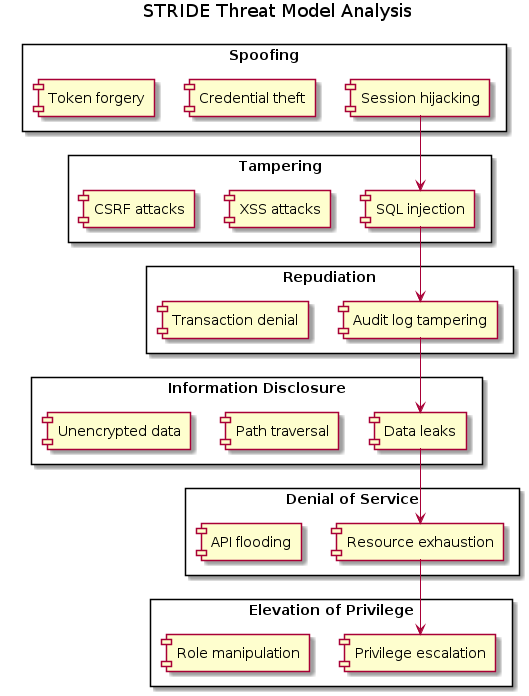
\includegraphics[width=0.7\textwidth]{images/stride-analysis}
	\caption{Visualizing Risk Assessment and Prioritization}
\end{figure}

\subsection*{4. Reporting Templates and Communication}
Standardized reporting templates are used to communicate risk findings and recommendations to stakeholders\cite{shostack2014}. These templates typically include:
\begin{itemize}
	\item Executive summary
	\item System overview and diagrams
	\item Threat and risk analysis tables
	\item Security control recommendations
	\item Action plan and timeline
\end{itemize}
Clear and consistent reporting ensures that decision-makers understand the risks and the steps being taken to mitigate them. Reports should be tailored to the audience, whether technical teams, business leaders, or regulators.

\subsection*{5. Continuous Improvement and Metrics}
Continuous improvement is the ongoing process of refining security practices based on lessons learned and evolving threats\cite{owasp}. Organizations integrate threat modeling into DevSecOps pipelines, schedule regular reviews and updates, track key metrics (such as the number of threats mitigated and time to remediation), and foster a security-aware culture through training and awareness. This adaptive approach ensures that risk management remains effective in the face of changing technologies and adversary tactics.
\begin{itemize}
	\item Integrate threat modeling into DevSecOps pipelines
	\item Schedule regular reviews and updates
	\item Track metrics (e.g., number of threats mitigated, time to remediation)
	\item Foster a security-aware culture through training and awareness
\end{itemize}

\subsection*{6. Academic Perspective and Further Reading}
For deeper understanding, refer to:
\begin{itemize}
	\item Adam Shostack, "Threat Modeling: Designing for Security" (Wiley, 2014)
	\item Tony UcedaVélez and Marco M. Morana, "Risk Centric Threat Modeling" (Wiley, 2015)
	\item NIST SP 800-154: Guide to Data-Centric System Threat Modeling
	\item OWASP Threat Modeling Cheat Sheet
\end{itemize}
